% !TEX root = catron-dissertation.tex
\epstopdfsetup{outdir=./images/01_introduction/}

\chapter{Introduction}
\label{chap:01_intro}

Directed-energy systems have a variety of uses but typically fall into one of two categories: communications and weapons.
The primary benefits of directed-energy communications is the ability to have secure point-to-point data transfer that is high unlikely to intercept or be interfered with \cite{crs-2021-RwNjGeZD}.
Directed-energy weapons are likely to have a lower cost per shot and a deeper magazine when compared to traditional munitions \cite{crs-2021-hyCUE868}.
As ground based directed-energy systems are slowly rolled out, most prominently aboard the USS Ponce \cite{crs-2021-Atxb7GDv}, there is a desire to field a system aboard an aircraft.

There have been two major attempts to field a directed-energy system aboard an aircraft to date \cite{Jumper-2013-8KtN3pue}.
The first was the Airborne Laser Laboratory (ALL) which took place in the late 1970's and early 1980's which used a CO$_2$ laser at 10.6-$\mu$m.
The second was the Airborne Laser (ABL) program which operated in the 2000's and used a COIL laser at 1.315-$\mu$m.
Airborne optical systems have to deal with a phenomenon know as ``aero-optics,'' which is optical distortions caused by various aero-dynamic flow features.
These optical distortions were first noticed due to image degradation in wind tunnel measurements in the 1950's \cite{Stine-1956-UaRzVZCe} as well as in photo-reconnaissance missions in the 1960's \cite{Kyrazis-2013-vwKeEBym}.

The intensity of that makes through an optical disturbance to a target, $I$, divided by the diffraction-limited performance, $I_0$, is known as the Strehl ratio \cite{Mahajan-1982-kkXM4eaB}, $\sr$,
\begin{equation}
  \sr = \frac{I}{I_0} \textrm{.}
  \label{eqn:01_strehl_ratio_definition}
\end{equation}
The diffraction-limited performance is the intensity that would make it to the same target if not for a disturbance.
The Airborne Laser Laboratory had an estimated Strehl ratio of 95\%\cite{Jumper-2013-8KtN3pue} meaning the ``aero-optics problem'' effectively did not apply.
After the Airborne Laser Laboratory program there was a desire to move toward shorter wavelengths in order to take advantage of improved diffraction-limited performance \cite{Jumper-2001-6QDh7zDy},
\begin{equation}
  \frac{I_0}{P} = \frac{1}{\pi}\left(\frac{Ap}{\lambda z}\right)^2 \textrm{,}
  \label{eqn:01_farfield_intensity}
\end{equation}
where $P$ is the laser output power, $Ap$ is the aperture size, and $z$ is the propagation distance.
This improved diffraction-limited performance is shown in Figure \ref{fig:01_farfield_intensity}.
\begin{figure}
  \centering
  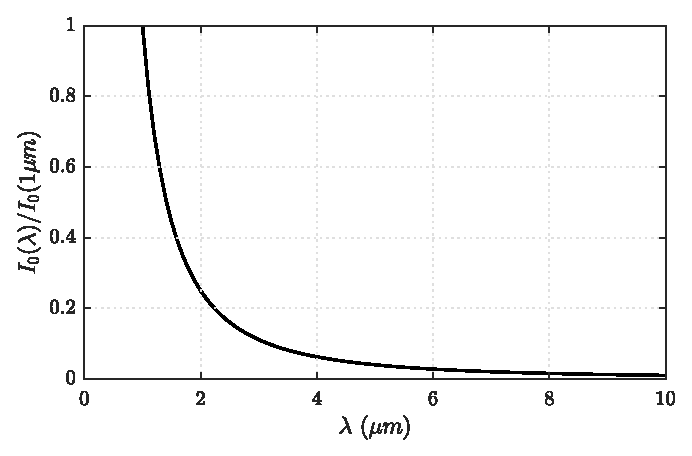
\includegraphics{../matlab/01_introduction/farfield_intensity.eps}
  \caption{Diffraction-limited far-field intensity of a beam normalized by the performance at 1-$\mu$m.}
  \label{fig:01_farfield_intensity}
\end{figure}
By only changing the laser source from a 10-$\mu$m to 1-$\mu$m wavelength the diffraction-limited performance can be increased 100 times.

Aero-optical issues start to become apparent as the wavelength is decreased as is evident by the Mar\'echal approximation \cite{Mahajan-1983-hg7ahvJM} which relates the Strehl ratio to wavelength,
\begin{equation}
  \sr \approx \exp\left\{-\left[\frac{2\pi \opdrms}{\lambda}\right]^2\right\} \textrm{,}
  \label{eqn:01_strehl_ratio}
\end{equation}
where $\opdrms$ is the spatial root-mean-square of the optical path difference over the aperture and is a way to quantify the optical disturbance that will be discussed in Chapter \ref{chap:02_lit_review}.
If the ALL system's laser was swapped with another laser of a lower wavelength, the Strehl ratio would significantly decrease as shown by Figure \ref{fig:01_strehl_ratio}.
\begin{figure}
  \centering
  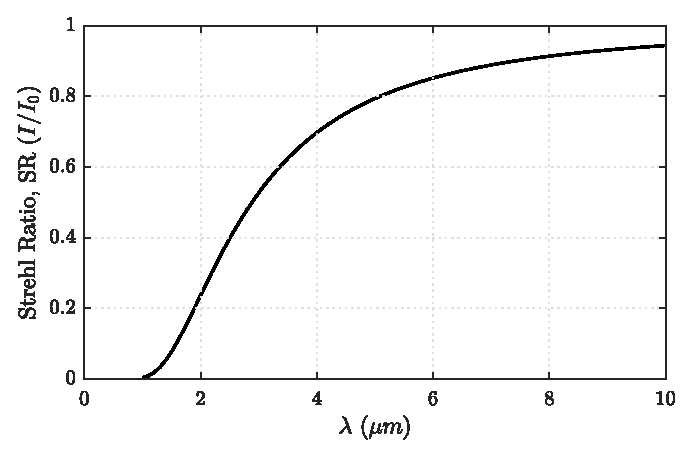
\includegraphics{../matlab/01_introduction/strehl_ratio.eps}
  \caption{Strehl ratio due to the $\opdrms$ of the Airborne Laser Laboratory (ALL) at various laser wavelengths.  ALL had an estimated Strehl ratio of 95\% with its 10.6-$\mu$m laser.}
  \label{fig:01_strehl_ratio}
\end{figure}
While the hypothetical case of going from 10 to 1-$\mu$m resulted in a 100-fold increase in diffraction-limited performance, the actual on-target intensity that this hypothetical system obtains would be essentially zero.
This means that the aero-optical problem can no longer be ignored and was recognized as one of the main developmental risks of the ABL program \cite{DOTE-1999-HnkadUEw}.
{\color{red}{Do you have or know of a source that at the very least alludes to the aero-optical issues with ABL that greatly limited its field of regard?}}

As the next generation of airborne directed-energy systems are developed some amount of ground testing of those systems will need to occur.
In order to understand the aero-optical environment that these systems will experience in the air wind tunnel tests will need to be employed.
These tests are far cheaper to perform and allow for quicker iteration of design parameters.
Wind tunnel tests will however include some additional optical contamination including but not limited to the boundary layer present on the wall and the acoustic environment generated by the wind tunnel fan \cite{Gordeyev-2014-jcJndkHM}.
Assuming that the optical disturbances system model are statistically independent from the optical disturbances from the testing environment, we can estimate the total optical disturbance from
\begin{equation}
  \opdrms_{TOTAL}^2 = \opdrms_{MODEL}^2+\opdrms_{ENVIRONMENT}^2 \textrm{.}
  \label{eqn:01_combined_opd}
\end{equation}

This combination of optical disturbances is shown in Figure \ref{fig:01_design_iteration} along with a hypothetical iterative design process.
\begin{figure}
  \centering
  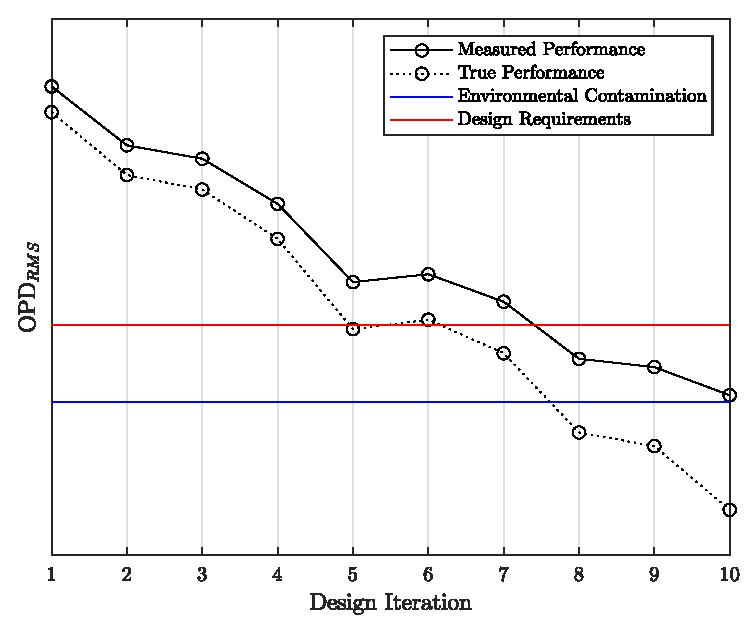
\includegraphics{../matlab/01_introduction/design_iteration.eps}
  \caption{Hypothetical iterative design process of an airborne directed-energy system.  The required performance level is shown by the red line and the testing environment's contamination is shown by the blue line.}
  \label{fig:01_design_iteration}
\end{figure}
This process seeks to obtain a design that meets a required level of performance shown in red.
If only the measured data is used to assess the system's performance three additional iterative changes are needed to achieve a usable design which can add significantly to the development time and costs.
If the environmental contamination is greater than the design requirement, the measured performance will never reach the required performance criteria.
When the true performance of a system is significantly higher than the environmental contamination, the measured performance is not significantly greater than the true performance.
The measured performance becomes significantly greater that the true performance when the true performance is less than the environmental contamination.

This dissertation will primary examine the environmental contamination due to acoustic noise within the wind tunnel.
In Chapter \ref{chap:03_optical_acoustics} it will look at the optical disturbances caused by acoustic waves from some simple plane and spherical waves to a process for estimating the acoustic environment within the test section of a wind tunnel.
The strength of an spherical acoustic wave will be assessed with both microphone and optical measurements.
Multi-dimensional spectral techniques will be used to analyze optical wavefronts in Chapter \ref{chap:04_dispersion} and filter optical wavefronts in Chapter \ref{chap:06_single_filter}.
These filtering techniques will contain some optical contamination particularly in regions where the various signal components interfere with one another.
In order to further reduce the optical contamination, Chapter \ref{chap:07_multiple_filter} will utilize additional sensor information from both microphones and accelerators to remove some of the overlapping contamination to obtain a better picture of the actual optical performance of an airborne directed-energy system from ground test measurements.
